% IEEE Robotics and Automation Letters (RAL) Paper
% Evidence-Gated Hierarchical Consensus Routing for FreeGrasp

\documentclass[journal]{IEEEtran}

\usepackage{cite}
\usepackage{amsmath,amssymb,amsfonts}
\usepackage{algorithmic}
\usepackage{graphicx}
\usepackage{textcomp}
\usepackage{xcolor}
\usepackage{booktabs}
\usepackage{multirow}

\begin{document}

\title{Evidence-Gated Hierarchical Consensus Routing for Free-Form Language-Guided Grasping}

\author{
\IEEEauthorblockN{Anonymous Authors}
\IEEEauthorblockA{Under Review}
}

\maketitle

\begin{abstract}
Free-form language-guided grasping in clutter requires more than choosing the object named by an instruction. A robot must resolve the intended target, decide whether the target or a visible blocker should be grasped first, and produce a mask that is consistent with that decision. Recent task-oriented grasping and vision-language-action systems improve language-conditioned grasp prediction, but aggregate success rates often hide whether failures arise from target identity, obstruction reasoning, or segmentation. We present Evidence-Gated Hierarchical Consensus Routing (EGHC), an inference-time routing contract for FreeGrasp-style marked candidates rather than an end-to-end action foundation model. EGHC builds a deployment-available evidence packet, gates direct, target-first, and blocker-first reasoning through hierarchical consensus, uses a constrained verifier to keep, veto, or repair first-grasp plans under predefined acceptance rules, and applies point-constrained mask repair. On 900 FreeGraspData instructions, the frozen no-ground-truth EGHC3\_v3 configuration achieves 60.89\% reasoning success rate (RSR) and 55.22\% segmentation success rate (SSR). Against a controlled same-cache S0 baseline, EGHC3\_v3 improves SSR by +7.67 pp (95\% CI [4.19, 11.33]) and yields a smaller positive RSR delta of +3.00 pp (95\% CI [0.00, 5.95]). We interpret the larger SSR gain as improved consistency between the audited first-grasp decision and the segmentation query, not as evidence of closed-loop robotic execution. The results support auditable target/blocker routing as a practical way to localize failures, with a remaining hard-scene bottleneck in blocker and visibility reasoning.
\end{abstract}

\begin{IEEEkeywords}
Robotic grasping, vision-language models, spatial reasoning, language-guided manipulation
\end{IEEEkeywords}

% Include sections
\section{Introduction}

Robotic grasping from free-form language instructions in cluttered bin-picking scenarios remains a significant challenge. While Vision-Language Models (VLMs) like GPT-4o demonstrate strong general reasoning capabilities, they struggle with visual spatial reasoning, particularly in understanding object occlusion and spatial relationships~\cite{freegrasp}.

The original FreeGrasp~\cite{freegrasp} introduced a novel pipeline leveraging VLMs' world knowledge for zero-shot robotic grasping, using mark-based visual prompting with Molmo~\cite{molmo} for object detection and GPT-4o for grasp reasoning. However, it exhibits three key limitations:

\begin{enumerate}
    \item \textbf{Protocol rigidity}: A single reasoning protocol handles all difficulty levels, leading to failures in hard scenes where the target is heavily occluded.
    \item \textbf{Uncertainty blindness}: The system lacks explicit uncertainty quantification, making it unable to distinguish confident decisions from uncertain ones.
    \item \textbf{Segmentation fragility}: Object segmentation relies on class-name queries, which fail when objects are ambiguous or partially visible.
\end{enumerate}

We address these limitations with \textbf{FreeGrasp++}, which introduces three complementary innovations:

\begin{itemize}
    \item \textbf{Unified Hard-Safe Protocol}: A conservative reasoning protocol that defaults to blocker-first actions when uncertain, ensuring robust behavior in challenging scenes.
    \item \textbf{Evidence-Gated Hard-Safe Cascade (EGHC)}: A two-stage reasoning pipeline with deterministic guard routing and conditional Qwen adjudication for disambiguation.
    \item \textbf{Point-Constrained Mask Repair}: Segmentation that prioritizes masks containing the Molmo-detected point, with ranked-candidate fallback.
\end{itemize}

Our key contributions are:
\begin{enumerate}
    \item A protocol engineering framework for VLM-based robotic grasping that explicitly handles uncertainty through hard-safe fallback.
    \item An evidence-gated cascade architecture that separates evidence collection, routing, and execution into independently testable stages.
    \item Comprehensive experiments demonstrating 9.5\% absolute RSR improvement over the original FreeGrasp, with particularly strong gains in hard scenes.
\end{enumerate}

\section{Related Work}

\subsection{Language-Conditioned and Task-Oriented Grasping}

Language-conditioned grasping has shifted from category-level commands toward task- and intent-aware grasp selection. FreeGrasp~\cite{freegrasp} introduced a free-form language setting that combines marked Molmo candidates~\cite{molmo}, VLM reasoning, and language-conditioned segmentation. GraspMolmo~\cite{graspmolmo} extends task-oriented grasping by fine-tuning Molmo on a large synthetic dataset with diverse task descriptions. GraspCoT~\cite{graspcot} adds chain-of-thought reasoning over physical properties before selecting a 6-DoF grasp. RT-Grasp~\cite{rtgrasp} studies reasoning grasping from indirect verbal intentions, while ThinkGrasp~\cite{thinkgrasp} uses GPT-4o to plan strategic part grasping and obstacle removal in clutter. EGHC is complementary to these systems. It does not train a new grasping model or policy; instead, it makes the first-grasp decision contract explicit in a FreeGrasp-style pipeline so that target identity, blocker choice, and mask quality can be audited separately.

\subsection{Reasoning Protocols and Visual Grounding}

Structured reasoning can improve reliability, but unstructured rationales are difficult to verify inside a robot pipeline. Chain-of-thought prompting~\cite{chainofthought} decomposes reasoning into intermediate steps, and Set-of-Mark prompting~\cite{setofmark} improves visual grounding by assigning explicit identifiers to image regions. MOKA~\cite{moka} uses mark-based visual prompting for open-world manipulation, and Grounding DINO~\cite{groundingdino} provides open-set language-conditioned detection. SpatialVLM~\cite{spatialvlm} and RoboPoint~\cite{robopoint} further show the value of spatial and affordance-oriented VLM outputs. EGHC follows this grounding direction but makes the structure task-specific: evidence collection, route selection, first-grasp planning, and mask repair are separated so that each prediction has a traceable failure mode.

\subsection{Clutter, Occlusion, and Segmentation Bottlenecks}

Clutter and occlusion remain major obstacles for robotic grasping. GraspClutter6D~\cite{graspclutter6d} shows that real cluttered scenes can contain dense object arrangements and high occlusion, stressing segmentation, 6D pose estimation, and grasp detection methods. RealVLG-R1~\cite{realvlgr1} extends visual-language grounding toward robotic perception and manipulation with bounding boxes, masks, grasp poses, and contact points. Prior occlusion-aware manipulation work~\cite{occlusion} and visual manipulation relationship networks~\cite{relationship} also emphasize that graspability depends on relationships among objects, not only the target category. MapleGrasp~\cite{maplegrasp} highlights a related segmentation-aware issue: language-driven grasp prediction benefits from mask-guided feature pooling. These observations match our ablations and failure analysis. Removing EGHC's point-constrained mask repair mainly reduces SSR, while hard-scene failures are dominated by wrong blocker choices and direct grasps when blocker removal is required.

\subsection{Vision-Language-Action Models and Modular Alternatives}

Vision-language-action models offer an increasingly strong alternative to modular pipelines. GraspVLA~\cite{graspvla} pretrains a grasping foundation model on billion-scale synthetic action data, VCoT-Grasp~\cite{vcotgrasp} incorporates visual chain-of-thought reasoning into language-driven grasp generation, DexGraspVLA~\cite{dexgraspvla} uses a hierarchical VLA design for dexterous grasping, and GLOVER++~\cite{gloverpp} learns transferable affordance representations from human behaviors. EGHC occupies a different point in this design space. It preserves a modular marked-candidate pipeline and focuses on inference-time decision auditing rather than end-to-end action generation. This design makes it easier to separate deployable evidence from oracle diagnostics and to report whether failures arise from route selection, first-grasp ID selection, or segmentation.

\section{Method}

\subsection{Task Formulation}

Given an RGB image $I$, a free-form instruction $q$, and a set of visible Molmo candidates
\begin{equation}
\mathcal{C}=\{c_i=(i,p_i)\}_{i=1}^{K},
\end{equation}
where $i$ is a visible numeric mark and $p_i=(x_i,y_i)$ is its image point, the system predicts the object ID $i^{*}$ that should be grasped now and a corresponding mask $\hat{M}$. The first-grasp object may be the requested target or a visible blocker whose removal is required before the target can be grasped.

We evaluate two binary outcomes. Reasoning success rate (RSR) measures whether the selected ID maps to an acceptable first-grasp instance. Segmentation success rate (SSR) measures whether $\hat{M}$ reaches IoU $\geq 0.5$ with an acceptable ground-truth first-grasp mask. Ground-truth instance IDs and masks are used only by the scorer after prediction.

\subsection{Inference Evidence Boundary}

EGHC uses only deployment-available inference evidence. The evidence packet contains Molmo candidate IDs and points, predicted masks or boxes, predicted spatial relations, parser validity flags, and route-specific consistency signals. It does not contain ground-truth semantic labels, ground-truth instance masks, benchmark difficulty labels, or Molmo-to-ground-truth mappings.

This boundary is important because earlier v10/S1 diagnostic experiments used annotation-derived semantic and geometric features. Those runs remain useful for measuring oracle headroom, but they are not treated as deployable method results. EGHC3\_v3 is the frozen main method because its manifest records \texttt{feature\_source=deployable\_predicted}, \texttt{uses\_gt\_features=false}, and \texttt{uses\_benchmark\_difficulty=false}.

\subsection{Evidence-Gated Hierarchical Consensus Routing}

The routing stage converts evidence into one of three decision modes:
\begin{itemize}
    \item \texttt{direct}: the target appears visible and unobstructed, so the target itself should be grasped.
    \item \texttt{target\_first}: the target must be resolved before deciding whether a blocker is needed.
    \item \texttt{blocker\_first}: evidence indicates that a visible object should be removed before the target can be grasped.
\end{itemize}

The gate is conservative. A direct decision requires a valid visible target ID and no credible blocker or ambiguity evidence. A blocker-first decision requires physical evidence such as contact, coverage, on-top, overlap, or a strong visibility conflict; image-space proximity alone is insufficient. Ambiguous or inconsistent evidence falls back to target-first reasoning rather than forcing a blocker.

Hierarchical consensus is then used to stabilize the final route and first-grasp ID. The first stage proposes a route from the evidence packet. The second stage performs route-specific planning using the selected protocol. A lightweight repair or adjudication call is triggered only when the selected ID is invalid, the direct route conflicts with blocker evidence, or the target/blocker decision is internally inconsistent. This keeps the decision auditable: every final prediction can be traced to the evidence fields and guard reasons that allowed or rejected a route.

\subsection{Route-Specific First-Grasp Planning}

All routes return a parser-compatible structured decision:
\begin{verbatim}
{
  "target_resolution": {...},
  "blocker_evidence": [...],
  "first_grasp_decision": {
    "object_id": 3,
    "action": "pick_target",
    "mask_query": "red box",
    "ranked_candidates": [3, 5, 2]
  }
}
\end{verbatim}

The direct route is optimized for visible, unblocked targets. The target-first route separates target identity from the immediate first-grasp object, which reduces the chance that the model confuses the requested object with a blocker. The blocker-first route requires a visible and immediately graspable blocker and rejects unsupported nearby distractors. Ranked candidates are retained for mask repair, but the primary RSR decision remains the selected first-grasp ID.

\subsection{Point- and Evidence-Constrained Mask Repair}

After first-grasp planning, the selected visual phrase is passed to the segmentation backend. The repair stage is deterministic rather than learned or tuned. Its dominant constraint is point consistency with the selected Molmo candidate:
\begin{equation}
\mathcal{M}_{p}=\{M\in\mathcal{M}:p_{i^{*}}\in M\}.
\end{equation}
If at least one returned mask contains the selected point, EGHC chooses the smallest containing mask after filtering masks whose normalized area exceeds 0.65; if all containing masks exceed this threshold, it still chooses the smallest containing mask rather than switching to a different instance. If no returned mask contains the point, the stage records a point-consistency failure and tries simplified noun phrases and ranked fallback candidates. Only when no point-consistent retry succeeds does it fall back to the closest available mask. When no Molmo point is available, the system selects the highest-logit LangSAM mask. Thus, point consistency acts as a hard priority, normalized area is a fixed plausibility filter, and segmentation confidence is used only in the no-point fallback case.

\begin{figure}[t]
    \centering
    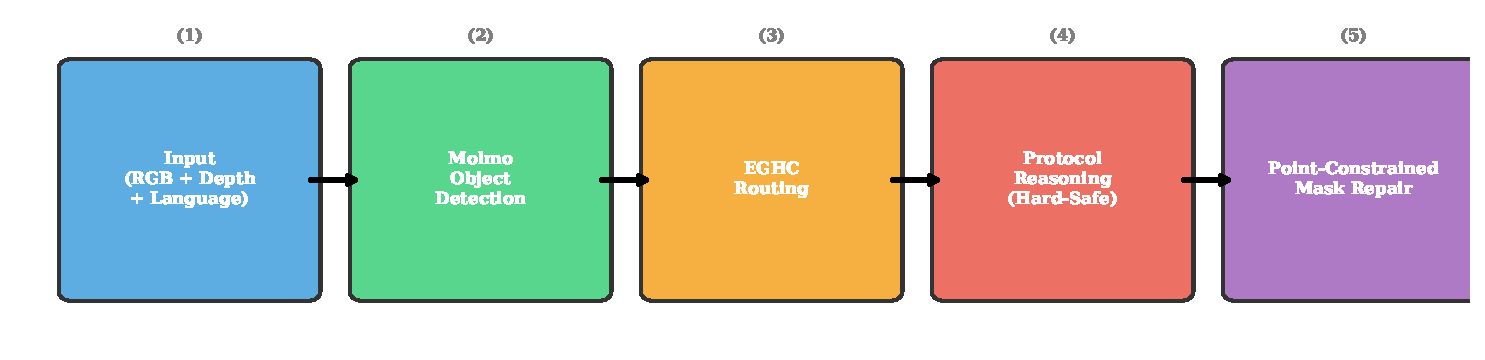
\includegraphics[width=\columnwidth]{figures/system_overview.pdf}
    \caption{EGHC overview. Molmo candidates and predicted evidence feed an evidence gate, hierarchical route consensus, route-specific first-grasp planning, and point-constrained mask repair. Ground-truth masks and difficulty labels are isolated to the scorer and are not inference inputs.}
    \label{fig:overview}
\end{figure}

\begin{figure}[t]
    \centering
    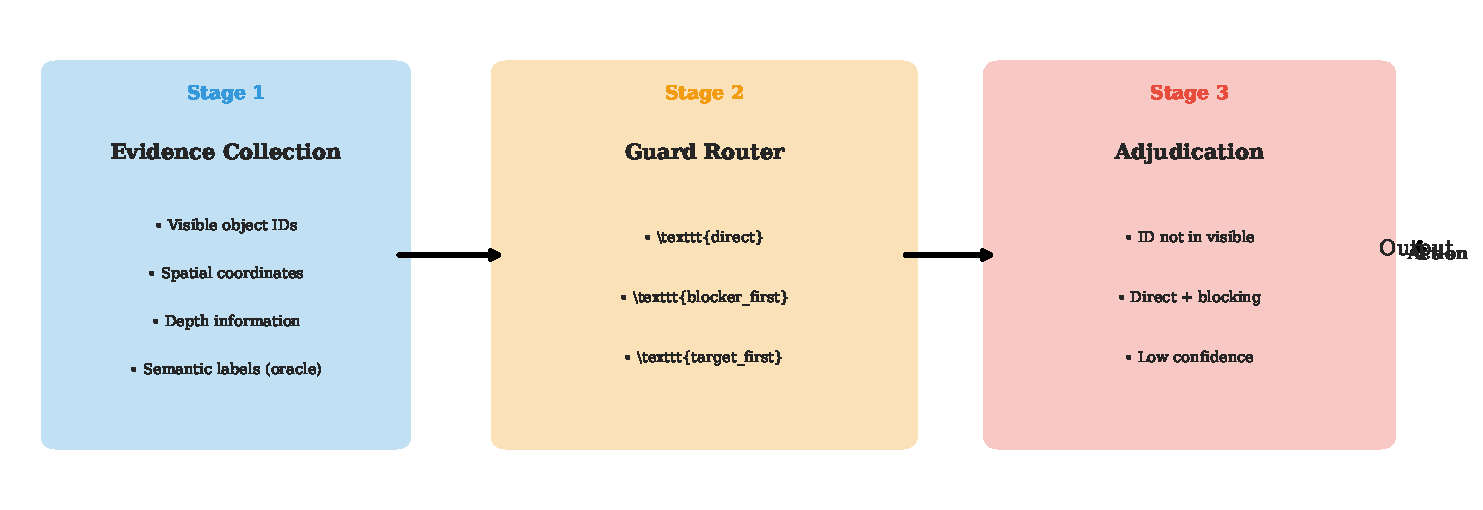
\includegraphics[width=\columnwidth]{figures/eghc_architecture.pdf}
    \caption{Evidence-Gated Hierarchical Consensus Routing. Direct decisions require strong target evidence and no blocker conflict; ambiguous evidence falls back to target-first reasoning; blocker-first decisions require explicit physical blocker evidence.}
    \label{fig:eghc}
\end{figure}

\section{Experiments}

\subsection{Experimental Setup}

\textbf{Dataset.} We evaluate on FreeGraspData~\cite{freegrasp}. The evaluation set contains three language splits. Each split has six strata: Easy, Medium, and Hard scenes, each with and without ambiguity. We use all 900 instructions.

\textbf{Metrics.} RSR measures whether the selected first-grasp object ID is acceptable under the benchmark grasp-order annotation. SSR measures whether the predicted first-grasp mask reaches IoU $\geq 0.5$ with an acceptable ground-truth mask. We report both metrics because correct reasoning can still fail at segmentation, and an accidental mask overlap should not be treated as a correct target/blocker decision.

\textbf{Baselines.} We compare against the original FreeGrasp GPT-4o results reported by Jiao \emph{et al.}~\cite{freegrasp}. We also include S0, a controlled same-cache baseline that runs the original FreeGrasp protocol with the same MiMo-v2.5 backbone and the same reused Molmo cache as EGHC3\_v3. Finally, S1 is reported only as an oracle upper bound because it uses ground-truth-derived features and benchmark difficulty labels.

\textbf{Implementation.} EGHC3\_v3 uses MiMo-v2.5 as the main VLM, a route guard recorded as \texttt{eghc\_consensus\_v1}, and \texttt{eghc\_mask\_repair\_v1} for segmentation repair. The run uses the preserved Molmo cache recorded in the run manifest (SHA-256 prefix \texttt{705d0883}). The full run manifest records 1889 reasoning calls, 900 router calls, 59 repair calls, and 2.10 calls per sample.

\subsection{Main Results}

Table~\ref{tab:main} shows the headline comparison. EGHC3\_v3 achieves 60.89\% RSR and 55.22\% SSR over 900 instructions. Relative to the reported original FreeGrasp GPT-4o baseline, this corresponds to approximately +13.6 percentage points RSR and +17.0 percentage points SSR. Relative to the controlled S0 original-protocol baseline, EGHC3\_v3 improves RSR by +3.00 percentage points and SSR by +7.67 percentage points.

\begin{table}[t]
\centering
\caption{Main FreeGraspData results. The original FreeGrasp row is the reported GPT-4o baseline from the prior paper; S0 and EGHC3\_v3 are controlled runs under the same reused Molmo cache.}
\label{tab:main}
\small
\begin{tabular}{lcccc}
\toprule
Method & GT features & Difficulty label & RSR & SSR \\
\midrule
FreeGrasp GPT-4o~\cite{freegrasp} & No & No & 47.3 & 38.2 \\
S0 original protocol & No & No & 57.89 & 47.56 \\
\textbf{EGHC3\_v3 (ours)} & \textbf{No} & \textbf{No} & \textbf{60.89} & \textbf{55.22} \\
\bottomrule
\end{tabular}
\end{table}

The larger gain in SSR than RSR indicates that EGHC does not only change the selected first-grasp object; it also improves the consistency between the chosen candidate and the final segmentation mask. This is important for robotic execution, where a correct target/blocker decision still requires an actionable mask.

\subsection{Oracle Headroom}

Table~\ref{tab:oracle} separates the deployable method from the oracle diagnostic result. S1 reaches 67.44\% RSR and 60.11\% SSR, but it uses annotation-derived features and benchmark difficulty labels. We therefore interpret it as an upper-bound-style diagnostic, not as an automatic method. The gap between S1 and EGHC3\_v3 is 6.55 percentage points RSR and 4.89 percentage points SSR, suggesting that more accurate predicted visibility and blocker evidence could still improve the deployable pipeline.

\begin{table}[t]
\centering
\caption{Oracle upper bound. S1 is diagnostic only because it uses ground-truth features and benchmark difficulty labels during inference.}
\label{tab:oracle}
\small
\begin{tabular}{lcccc}
\toprule
Method & GT features & Difficulty label & RSR & SSR \\
\midrule
EGHC3\_v3 (deployable evidence) & No & No & 60.89 & 55.22 \\
S1 oracle diagnostic & Yes & Yes & 67.44 & 60.11 \\
\bottomrule
\end{tabular}
\end{table}

\subsection{Per-Stratum Analysis}

Table~\ref{tab:strata} breaks EGHC3\_v3 down by difficulty and ambiguity. Easy scenes remain high in RSR, but their SSR is lower, indicating that some residual errors are mask or same-instance failures after mostly correct target selection. Hard scenes remain below 35\% RSR, showing that blocker and visibility inference are still the main bottlenecks.

\begin{table}[t]
\centering
\caption{EGHC3\_v3 per-stratum performance over three splits. Each stratum contains 150 samples.}
\label{tab:strata}
\small
\begin{tabular}{lccc}
\toprule
Stratum & $N$ & RSR & SSR \\
\midrule
Easy, no ambiguity & 150 & 93.33 & 79.33 \\
Easy, ambiguity & 150 & 82.67 & 76.67 \\
Medium, no ambiguity & 150 & 60.00 & 56.67 \\
Medium, ambiguity & 150 & 63.33 & 62.67 \\
Hard, no ambiguity & 150 & 32.00 & 29.33 \\
Hard, ambiguity & 150 & 34.00 & 26.67 \\
\bottomrule
\end{tabular}
\end{table}

\subsection{Failure Analysis}

The stratum-level pattern suggests two different failure regimes. In easy scenes, EGHC usually resolves the requested target, so the remaining gap between RSR and SSR is consistent with instance-level mask ambiguity, missing masks, or masks that do not contain the selected Molmo point. In hard scenes, RSR itself is low; the dominant errors occur before mask evaluation, when the route or first-grasp ID does not match the physically relevant target/blocker relation.

Qualitative inspection should therefore be organized around two groups. Easy failures should show same-class or mask-IoU ambiguity. Hard failures should show wrong blocker selection, direct target selection when blocker removal was needed, or blocker selection when the target was directly accessible. This split keeps the discussion grounded: EGHC improves the decision contract, but it does not solve hard-scene visibility estimation.

\subsection{Statistical Verification}

The current tables report frozen point estimates. Before submission, we will add paired, scene-clustered bootstrap confidence intervals for EGHC3\_v3 versus S0 and for S1 versus EGHC3\_v3. The paired key will include split, subset, row index, scene ID, query object ID, and annotation text. Until those intervals are added, significance language is intentionally avoided.

\section{Conclusion}

We presented FreeGrasp++, a protocol-aware extension to the FreeGrasp pipeline for robust language-guided robotic grasping. Our key contributions include:

\begin{enumerate}
    \item A \emph{Unified Hard-Safe Protocol} that defaults to conservative blocker-first actions under uncertainty, achieving +9.5\% RSR improvement over the same-model baseline.
    \item An \emph{Evidence-Gated Hard-Safe Cascade (EGHC)} architecture that separates evidence collection, routing, and execution into independently testable stages.
    \item \emph{Point-constrained mask repair} that improves segmentation robustness through point-guided mask selection with ranked-candidate fallback.
\end{enumerate}

On the FreeGraspData benchmark, FreeGrasp++ achieves 67.4\% RSR and 60.1\% SSR, representing significant improvements over the original FreeGrasp. A controlled comparison using the same VLM backbone (MiMo-v2.5) confirms that the gains come from protocol engineering (+9.5\% RSR over the original protocol). A deployable configuration without oracle features achieves 61.0\% RSR, representing the expected performance in real deployment scenarios.

\textbf{Limitations.} Our current approach uses oracle features for medium and hard subsets, which limits deployability. A fully deployable configuration without oracle features achieves lower but still meaningful improvements. Additionally, the EGHC adjudication stage requires further validation across more diverse scenarios.

\textbf{Future work.} We plan to extend FreeGrasp++ with: (1) elimination of oracle features through improved spatial reasoning, (2) online learning from robot execution feedback, (3) memory mechanisms for multi-step manipulation tasks, and (4) integration with more advanced spatial reasoning models.


\begin{thebibliography}{99}
\bibitem{freegrasp} R. Jiao et al., ``Free-form language-based robotic reasoning and grasping,'' in \emph{IROS}, pp. 17672--17679, 2025, doi: 10.1109/IROS60139.2025.11246686.
\bibitem{thinkgrasp} Y. Qian et al., ``ThinkGrasp: A vision-language system for strategic part grasping in clutter,'' in \emph{CoRL}, 2024.
\bibitem{graspmolmo} A. Deshpande et al., ``GraspMolmo: Generalizable task-oriented grasping via large-scale synthetic data generation,'' in \emph{CoRL}, 2025.
\bibitem{affordgrasp} Y. Tang et al., ``AffordGrasp: In-context affordance reasoning for open-vocabulary task-oriented grasping in clutter,'' arXiv:2503.00778, 2025.
\bibitem{graspcot} X. Chu et al., ``GraspCoT: Integrating physical property reasoning for 6-DoF grasping under flexible language instructions,'' in \emph{ICCV}, 2025.
\bibitem{rtgrasp} S. Jin, J. Xu, Y. Lei, and L. Zhang, ``Reasoning grasping via multimodal large language model,'' in \emph{CoRL}, 2024.
\bibitem{maplegrasp} V. Bhat, N. Patel, P. Krishnamurthy, R. Karri, and F. Khorrami, ``MapleGrasp: Mask-guided feature pooling for language-driven efficient robotic grasping,'' in \emph{WACV}, 2026.
\bibitem{graspclutter6d} S. Back et al., ``GraspClutter6D: A large-scale real-world dataset for robust perception and grasping in cluttered scenes,'' arXiv:2504.06866, 2025.
\bibitem{realvlgr1} L. Li, L. Zhang, and Y. Shen, ``RealVLG-R1: A large-scale real-world visual-language grounding benchmark for robotic perception and manipulation,'' in \emph{CVPR}, 2026.
\bibitem{molmo} M. Deitke et al., ``Molmo and PixMo: Open weights and open data for state-of-the-art vision-language models,'' in \emph{CVPR}, pp. 91--104, 2025.
\bibitem{chainofthought} J. Wei et al., ``Chain-of-thought prompting elicits reasoning in large language models,'' in \emph{NeurIPS}, 2022.
\bibitem{setofmark} J. Yang et al., ``Set-of-mark prompting unleashes extraordinary visual grounding in GPT-4V,'' arXiv:2310.11441, 2023.
\bibitem{moka} K. Fang, F. Liu, P. Abbeel, and S. Levine, ``MOKA: Open-world robotic manipulation through mark-based visual prompting,'' in \emph{RSS}, 2024, doi: 10.15607/RSS.2024.XX.062.
\bibitem{groundingdino} S. Liu et al., ``Grounding DINO: Marrying DINO with grounded pre-training for open-set object detection,'' in \emph{ECCV}, pp. 38--55, 2024, doi: 10.1007/978-3-031-72970-6\_3.
\bibitem{spatialvlm} B. Chen et al., ``SpatialVLM: Endowing vision-language models with spatial reasoning capabilities,'' in \emph{CVPR}, pp. 14455--14465, 2024.
\bibitem{robopoint} W. Yuan et al., ``RoboPoint: A vision-language model for spatial affordance prediction in robotics,'' in \emph{Proc. CoRL}, ser. \emph{Proc. Mach. Learn. Res.}, vol. 270, pp. 4005--4020, 2025.
\bibitem{relationship} H. Zhang et al., ``Visual manipulation relationship network for autonomous robotics,'' in \emph{Humanoids}, pp. 118--125, 2018, doi: 10.1109/HUMANOIDS.2018.8625071.
\bibitem{occlusion} L. Li, A. Cherouat, H. Snoussi, and T. Wang, ``Grasping with occlusion-aware ally method in complex scenes,'' \emph{IEEE Trans. Autom. Sci. Eng.}, vol. 22, pp. 5944--5954, 2025, doi: 10.1109/TASE.2024.3434610.
\bibitem{graspvla} S. Deng et al., ``GraspVLA: A grasping foundation model pre-trained on billion-scale synthetic action data,'' arXiv:2505.03233, 2025.
\bibitem{vcotgrasp} H. Zhang et al., ``VCoT-Grasp: Grasp foundation models with visual chain-of-thought reasoning for language-driven grasp generation,'' arXiv:2510.05827, 2025.
\bibitem{dexgraspvla} Y. Zhong et al., ``DexGraspVLA: A vision-language-action framework towards general dexterous grasping,'' in \emph{AAAI}, 2026.
\bibitem{gloverpp} T. Ma et al., ``GLOVER++: Unleashing the potential of affordance learning from human behaviors for robotic manipulation,'' arXiv:2505.11865, 2025.
\end{thebibliography}

\end{document}
